% This is LLNCS.DEM the demonstration file of
% the LaTeX macro package from Springer-Verlag
% for Lecture Notes in Computer Science,
% version 2.4 for LaTeX2e as of 16. April 2010
%
\documentclass{article}
%
\usepackage{makeidx}  % allows for indexgeneration
\usepackage{amsmath}
\usepackage{graphicx}
\usepackage{color}
\usepackage{transparent}
\usepackage{pbox}
\usepackage{pgfplots}
\usetikzlibrary{calc} 
\pgfplotsset{compat=1.8}
%\usepackage{array}
%
\begin{document}

%
\pagestyle{headings}  % switches on printing of running heads
%\addtocmark{Hamiltonian Mechanics} % additional mark in the TOC
%
%\tableofcontents
%

%

\title{Automatic length and angle calculation of DNA on AFM images}

\author{Insert authors' names here}

\maketitle  
\newpage
\tableofcontents
\newpage
%
\begin{abstract}
This report summarizes ...

\end{abstract}

\section{Introduction}
This is how you cite \cite{ficarra2005automated}.
The sources are saved in sources.bib. If you find a paper/article/book on googlescholar, click "cite" and copy the bibtex cite style into the source file. It will looks something like this:
\begin{verbatim}
@article{ficarra2005automated,
  title={Automated DNA fragments recognition and sizing through AFM image processing},
  author={Ficarra, Elisa and Benini, Luca and Macii, Enrico and Zuccheri, Giampaolo},
  journal={Information Technology in Biomedicine, IEEE Transactions on},
  volume={9},
  number={4},
  pages={508--517},
  year={2005},
  publisher={IEEE}
}
\end{verbatim}
Alternatively just save them in a text document and we will merge all of them in the end. 

\subsection{Related Work}


The analysis of AFM images can be categorized into manual, semi-automatic and automatic approaches. Since the manual image analysis where human operators draw manually the backbone of DNA filaments is very time consuming and error-prone, we focused on a fully automatic analysis without any supervision. In semi-automatic analysis approaches, the threshold had been set manually or the initial and/or final point of a DNA filament was set by a human operator \cite{wiggins2006high}, \cite{marek2005interactive}, \cite{cassina2016effects}.

The automatic analysis predominantly focussed on the determination of the contour length of DNA filaments \cite{spisz1998automated}, \cite{sanchez2002accuracy}, \cite{sundstrom2012image}, \cite{marturelliautomated}. The sequences of the algorithms are in most points very similar and will be explained in the following step by step. The contour length is defined as the polymer’s length at maximal physical extension \cite{rivetti2001accurate}.  Some research groups also considered the curvature or the spatial orientation of DNA filaments \cite{ficarra2005automated}, \cite{ficarra2005automatic}. DNA-protein interactions such as in our approach the interaction between histones and DNA has not been automatically analysed so far. 
The main steps of DNA contour length determination are first the generation of a binary image, then the skeletonization of traced DNA fragments and then the length measurement. Many papers are referring to additional optional steps which are not necessary depending on which algorithms were implemented for the thinning step. In the following section the single steps of the algorithms are explained. 

\subsubsection{Filtering}
In order to reduce the noise, one apply filters before generating the binary image. The filters are either 3x3 mean filters \cite{rigotti2005quantitative} or 3x3 median filters \cite{ficarra2005automatic}, \cite{ficarra2002automated} which is extended by Ficarra et al. by a Gaussian filter and an adaptive filter \cite{ficarra2005automated}. 

\subsubsection{Segmentation}
The generation of a binary image is based on a thresholding algorithm which is either setting the threshold globally or locally, depending on the restriction of the method. Global thresholds are only including the grey values of a pixel whereas in local thresholding, the neighbourhood of a pixel is critical as well \cite{weszka1978survey}. Since local thresholding methods are very CPU-intensive, most studies use global thresholding algorithms. Their thresholds mostly depend on the pixels’ intensity values, whereas in one case a global size threshold of 0.2 nm was set \cite{sanchez2002accuracy}. Finding the optimal threshold where only valid fragments and no background are considered is a challenging task. Ficarra et al. use the Ridler method, a method based on a grey histogram which iteratively determines the optimal threshold \cite{ridler1978picture}. Spisz et al. use two different thresholding techniques. The first technique is based on two Gaussian distributions fitted to the fore- and background grey values and finds the optimal threshold in between those distributions \cite {gonzales1987wintz}. The algorithm cannot be applied to all AFM images, therefore they implemented a second method which finds the minimum threshold where the number of recognized fragments (blobs) does not change \cite{russ1992image}. Setting a too high threshold leads to the fragmentation of DNA filaments (see figure \ref{fig: blobs}.

\begin{figure}[htb]
\begin{center}
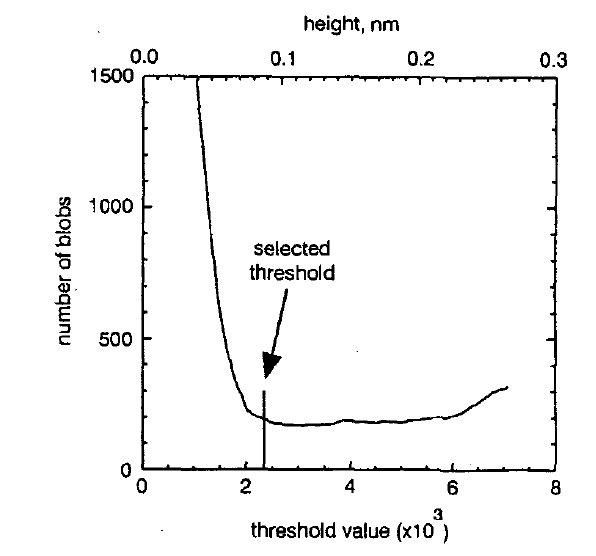
\includegraphics[width = 0.7\textwidth]{Segmentation_histo}
\end{center}
\caption{Determination of optimal threshold. For each threshold the resulting number of blobs have been calculated. The optimal threshold is the minimal threshold value at which the number of blobs does not decrease any further.\cite{russ1992image}}
\label{fig: blobs} % you need to include this to reference the figure afterwards
\end{figure}

Another option is to consider a pixel’s neighbouring intensity values instead of the pixel’s intensity value \cite{marek2005interactive}. By doing so, filtering and segmentation are taken together into one step.


\subsubsection{Thinning}
The thinning step is included in order to erode the fragments to skeletons with the width of one pixel which is necessary for the length determination. The fast parallel thinning algorithm by Zhang and Suen iteratively removes pixels from each fragment if they possess all the conditions of removal \cite{ficarra2005automated}, \cite{ficarra2002automated}, \cite{ficarra2005automatic}, \cite{spisz1998automated}, \cite{zhang1984fast}, \cite{marturelliautomated}. This algorithm does not include the removal of corner pixels and has high probability to remove valid end pixels. The algorithm by Brugal and Chassery however iteratively removes connected pixels in a specific order and thereby ensures that no pixel return is necessary \cite{brugal1977new}, \cite{sanchez2002accuracy}. Sundstrom et al. do not name their thinning algorithm but only emphasize that it is necessary to convert the fragments into skeletons with a width of one pixel \cite{sundstrom2012image}.


\subsubsection{Removal of corner Pixel}

During thinning invalid corner pixels can be included which results in a longer distance in corner areas. Those pixels are not real compartments of the DNA structure and hence need to be removed \cite{sanchez2002accuracy}, \cite{ficarra2002automated}, \cite{spisz1998automated}.

\subsubsection{Removal of objects across the image boundary}

For fragments at the image boundary no complete analysis is possible. Therefore, they have to be excluded from further steps. Ficarra et al. used an 8-pixel neighbourhood for the detection of such objects. If the blob connectivity was not interrupted at the image boundary the object has been removed \cite{ficarra2005automated}, \cite{ficarra2005automatic}. 

\subsubsection{Pruning}

After thinning some short branches remain at the skeletons. They come from impurities in the sample or from noise close to the DNA fragment. Sundstrom et al. referred to a master thesis by Silvio Civonne who transformed the skeleton into a graph. Thereby it was no more an image optimization problem but a graph optimization problem \cite{sundstrom2012image}. Otherwise, the removal of the branch pixels is necessary. Ficarra et al. created a mask which is able to distinguish between good cases, branches, critical cases and corners. Spurious branches have the characteristic of being much shorter than the fragment. This feature is used to identify such branches and to delete them recursively \cite{ficarra2002automated}, \cite{ficarra2005automated}.  



\subsubsection{Removal of invalid fragments}

In this step, critical molecules are removed before analysing their length. Spisz et al. carry out this step before thinning the fragments. Fragments are defined as invalid when they are overlapping with other fragments or with themselves, when they are in a closed circle conformation, when the endpoints are not distinguishable, when more than two endpoints are detected and when they overstep a user-defined size \cite{spisz1998automated}, \cite{ficarra2005automated}, \cite{ficarra2002automated}, \cite{ficarra2005automatic}. Ficarra et al. used for the removal of such invalid fragments different masks. For overlapping molecules the masks shown in figure \ref{fig: Masken} have been used \cite{ficarra2005automated}.

\begin{figure}[htb]
\begin{center}
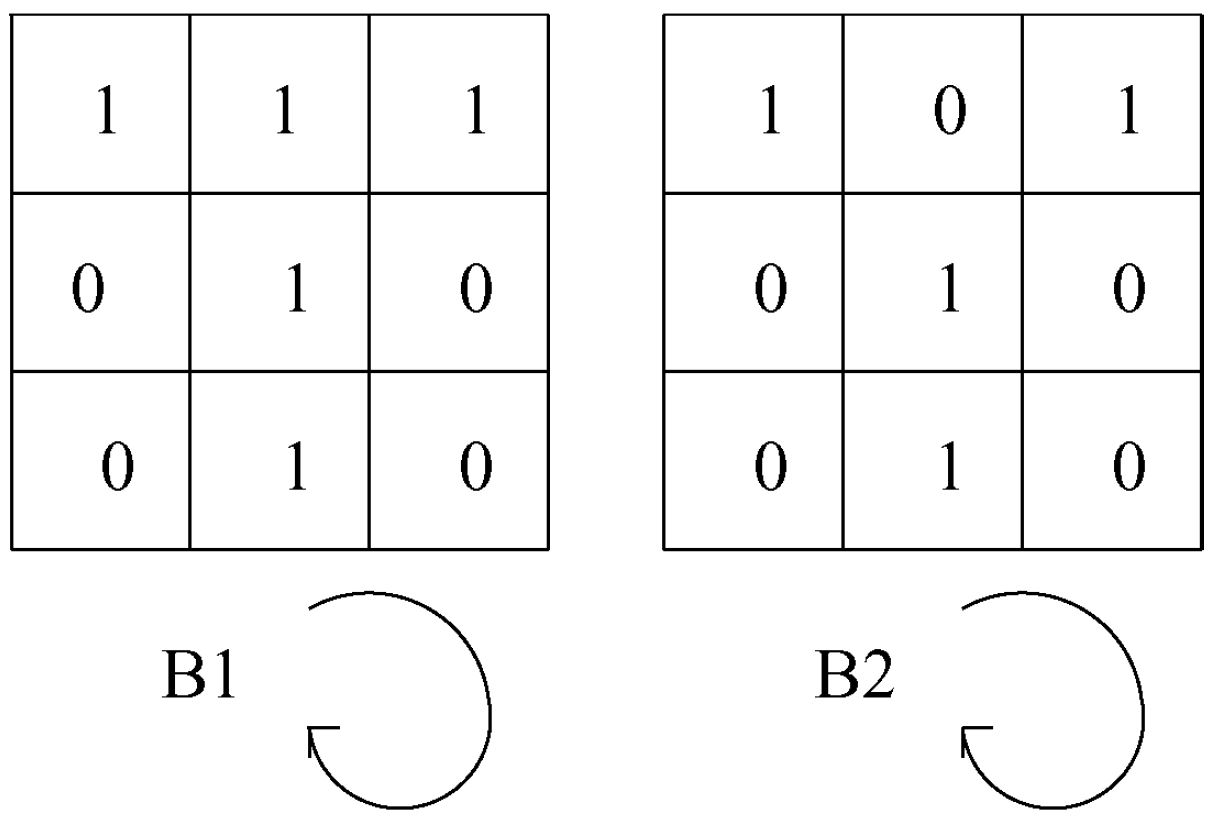
\includegraphics[width = 0.7\textwidth]{Masken}
\end{center}
\caption{Masks for identifying overlapping molecules.\cite{ficarra2002automated}}
\label{fig: Masken} % you need to include this to reference the figure afterwards
\end{figure}



\subsubsection{Pixel restoring}

Pixel at the skeleton ends only need to be restored if they were erroneously deleted during thinning of the fragment. The end pixels of each backbone are virtually extended in the direction of the last two pixels. If the new possible end point was part of the fragment before, the pixel is restored \cite{spisz1998automated}, \cite{ficarra2005automated}, \cite{ficarra2002automated}, \cite{ficarra2005automatic}.



\subsubsection{Length determination}

The determination of the length of the DNA skeletons is achieved by estimating the contour length which is defined as the polymer’s length at maximal physical extension \cite{rivetti2001accurate}.  During digital processing, the exact contour is lost. Anyhow, the accurate determination of the contour length is for many applications crucial. The Freeman estimator is the most commonly used method to determine the length \cite{spisz1998automated}, \cite{marturelliautomated}. When the fragment is reduced to a skeleton with the width of one pixel, the connection between one and another pixel can be represented by eight directions (figure \ref{fig: freeman}A). The Freeman estimator is adding the distance between the connected pixels from one endpoint to another. Even connections thus with vertical or horizontal direction are counting as 1, odd connections with diagonal connections are multiplied by 1.414. \\

$ L_{F} = n_{e} + \sqrt{2n_{o}} = 1.000n_{e} + 1.414n_{o}  $ 

\hspace{0,2cm}
 
$ L_{F}$: \begin{footnotesize} 
DNA contour length determined by the Freeman estimator
\end{footnotesize}  

$ n_{e}$: \begin{footnotesize} 
 number of even connections
\end{footnotesize} 
 
$ n_{c}$: \begin{footnotesize} 
 number of odd connections
\end{footnotesize}  \\

Even though the Freeman estimator is often favoured, it overestimates the DNA length with approximately eight percent \cite{sanchez2002accuracy}. Rivetti and Codeluppi analysed in 2001 six different algorithms to determine the contour length, one of them being the Freeman estimator. 
Secondly, they tested the most probable origin estimator, which similar to the Freeman estimator computes an ($n_{e}$, $n_{o}$) characterization. \\

$ L_{MPO} = \sqrt{(n_{e} + n_{o})^{2} + n_{e}^{2}} $

\hspace{0,2cm}

$ L_{MPO} $: \begin{footnotesize}
DNA contour length determined by the most probable origin estimator
\end{footnotesize} \\

They gained much better results for the Kulpa estimator which is derived from the Freeman estimator. The Coefficients of even and odd pixels minimize the error when measuring the length long fragments.\\

$ L_{K} = 0.948n_{e} + 1.343 n_{o} $

\hspace{0,2cm}

$ L_{k} $: \begin{footnotesize}
DNA contour length determined by the Kulpa estimator
\end{footnotesize} \\

The corner count estimator considers additionally to the number of even and odd connections the number of different code pairs, so called corners (figure \ref{fig: freeman}B) \cite{vossepoel1982vector}. The coefficients were found by least-square fitting \cite{yang1994methods}.  \\


$ L_{C} = 0.980n_{e} + 1.406 n_{o} - 0.091 n_{c} $

\hspace{0,2cm}

$ n_{c} $: \begin{footnotesize}
number of corners
\end{footnotesize} \\


\begin{figure}[htb]
\begin{center}
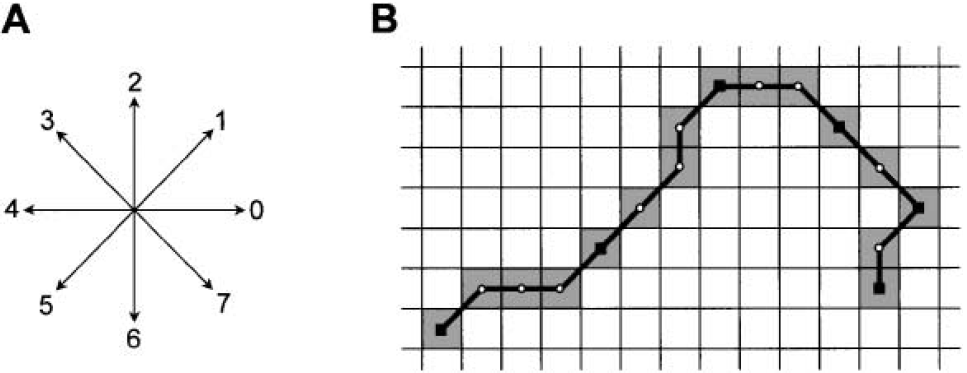
\includegraphics[width = 0.7\textwidth]{freeman}
\end{center}
\caption{(A) Scheme of the eight connected chain code. (B) Example of a fragment skeleton containing 16 pixels (grey grid elements). The chain is connected by 15 codes, from the left to the right chain the codes can be written as 100111210077756. There are six even codes ($ n_{e} $) and nine odd codes ($ n_{o} $). The total number of corners ($ n_{c}$) is six.}
\label{fig: freeman} % you need to include this to reference the figure afterwards
\end{figure}

As fourth estimator Rivetti and Codeluppi tested an estimator where the backbone was primarily smoothed by using polynomial fitting. The coordinates of each pixel where thereby adjusted. The polynomial degree was three and the moving window consisted of five points since the estimation with this combination were very close to the real length. \\ 

$ L_{PF} = \sum_{i=1}^{n-1} \sqrt{(x_{i+1}-x_{i})^{2} + (y_{i+1}-y_{i})^{2}} $

\hspace{0,2cm}

$ L_{PF} $: \begin{footnotesize}
DNA contour length determined with polynomial smoothing
\end{footnotesize} \\



The last algorithm included in their analysis was the edge chain algorithm which was originally implemented to measure the length of the roots of plants. It can be applied for other objects with relatively constant width and draws chords along the object edge to determine its perimeter. \\

$ L_{ECA}=\dfrac{P+\sqrt{P^{2}-16A}}{4} $

\hspace{0,2cm}

$ L_{ECA} $: \begin{footnotesize}
DNA contour length determined by the edge chain algorithm 
\end{footnotesize} 

$ P $:\begin{footnotesize}
perimeter
\end{footnotesize} 

$ A $:\begin{footnotesize}
area
\end{footnotesize} \\

Rivetti and Codeluppi generated synthetic data similar to their AFM images with DNA fragments of different length and tested the estimators while knowing the exact length of the synthetic filaments. The estimations with the Kulpa estimator, the corner count estimator and with polynomial smoothing were significantly closer to the real length of the filaments than the estimates generated by the other three estimators. The overestimation of the Freeman estimator was confirmed \cite{rivetti2001accurate}.



Ficarra et al. calculated the molecule length using the Euclidean distance which was integrated over all consecutive pixels of the molecule. For calculation the pixel coordinates were recalculated as weighed average by the usage of a weight factor k.\\


$ X_{P} = k(x_{p-1}-x_{p})+x_{p}+k(x_{p+1}-x_{p}) $

$ L_{P+1,p}= \sqrt{(X_{p+1}-X_{p})^{2}+(Y_{p+1}-Y_{p})^{2}} $

\hspace{0,2cm}

$ X_{P} $:\begin{footnotesize}
weighed average x coordinate
\end{footnotesize}

$ k $:\begin{footnotesize} 
single weight factor
\end{footnotesize}

$ L_{p+1,p} $:\begin{footnotesize} 
modified distance between the points with coordinates x and y
\end{footnotesize}\\






\section{Methods}
This is how you include tables:
\begin{table}[htb]
\begin{center}
\caption{My Table Caption.}
\label{tab: example} % you need to include this to reference the table afterwards
\begin{tabular}{|l|l|l|l|l|l|}
\hline
x & y & z & $\alpha$
& $\beta$
& $\gamma$\\\hline
30 & 0.82 & 38.4 & 35.7 & 154 & 320 \\
60 & 0.67 & 42.1 & 34.7 & 138 & 340 \\
120 & 0.52 & 45.1 & 34.0 & 124 & 370 \\
\hline
\end{tabular}
\end{center}
\end{table}\\
And this is how you reference a table: See Table \ref{tab: example}.\\
\newpage

This is how you include figures:
%\begin{figure}[htb]
%\begin{center}
%\includegraphics[width = 0.7\textwidth]{041.png}
%\end{center}
%\caption{My Figure Caption.}
%\label{fig: example} % you need to include this to reference the figure afterwards
%\end{figure}

This is how you reference a Figure: See Figure \ref{fig: example}. \\
And this is how you reference a section: See Section \ref{sec: Results}.
\subsection{Software Architecture}
\subsection{Algorithm}
\subsection{Optimization}
\subsection{Test Data Creation}
\section{Results}\label{sec: Results}
\subsection{Validation}
\subsection{Biological Significance}
\section{Discussion}
\section{Conclusion and Outlook}

\section{References}
%
\bibliography{sources}
\bibliographystyle{plain}

\end{document}
